\documentclass[12pt,letterpaper]{article}
\usepackage[utf8]{inputenc}
\usepackage[spanish,es-tabla]{babel}
\decimalpoint
\let\cleardoublepage\clearpage
\usepackage[bitstream-charter]{mathdesign} 
\usepackage[T1]{fontenc}
\newcommand{\selectSans}{\usefont{T1}{qhv}{m}{n}\selectfont} % sans-serif TeX Gyre Heros font
\usepackage{amsmath}
\usepackage{amsfonts}
\usepackage{amssymb}
% \usepackage[T1]{fontspec}
\usepackage{color}
\usepackage{graphicx}
\usepackage{makeidx}
\usepackage{textcomp}
\usepackage{gensymb}
\makeindex
\usepackage{enumitem}
\usepackage{anysize}
\usepackage{anyfontsize}
\usepackage{pdfpages}
\usepackage[x11names,table]{xcolor}
\usepackage{tikz}
\usepackage{tcolorbox}
\tcbuselibrary{skins,breakable,listings,theorems}
\usepackage[hidelinks]{hyperref}
\usepackage[labelfont=bf]{caption}
\captionsetup[table]{labelsep=space}
\captionsetup[figure]{labelsep=space}
\usepackage{listings}
\usepackage{array,ragged2e}
\usepackage{multirow}
\usepackage[left=2.5cm,top=2cm,right=2.5cm,bottom=2cm]{geometry}
\setlength{\parindent}{0cm}
\usepackage[printwatermark]{xwatermark}
\newwatermark[allpages,color=gray!10,angle=45,scale=3,xpos=0,ypos=0]{Borrador}

\tcbset{colback=green!5!white, colframe=gray!10!black, coltitle=green!20!black, 
fonttitle=\bfseries, colbacktitle=white, coltext=gray!30!black}
\addto\captionsspanish{
  \renewcommand{\figurename}{{\bf Figura}}% 
}
\addto\captionsspanish{
  \renewcommand{\chaptername}{{\bf}}% 
}

\usepackage{epigraph}
\usepackage{fontawesome}
\usepackage[Bjornstrup]{fncychap}

% \renewcommand{\familydefault}{\sfdefault}

% Colores
\definecolor{verdep}{RGB}{166,206,58}
\definecolor{ccap}{RGB}{10,10,50}
\definecolor{csec}{RGB}{50,50,100}
\definecolor{csubsec}{RGB}{80,80,120}
\definecolor{header_table_color}{RGB}{200,255,180}
\definecolor{info_color}{RGB}{100,100,200}
\definecolor{csol}{rgb}{0.2,0.8,0.1}
\definecolor{backcode}{rgb}{0.98,0.98,0.99}
\definecolor{crule}{rgb}{0.9,0.9,0.9}
\definecolor{dkgreen}{rgb}{0,0.6,0}
\definecolor{gray}{rgb}{0.5,0.5,0.5}
\definecolor{mauve}{rgb}{0.58,0,0.82}


\newtcolorbox{ejemplo}[2][]
{
  breakable,
  colframe = gray!50,
  colback  = gray!0,
  coltitle = gray!20!black,
  title    =  \faEdit \hspace{5 mm} #2,
}

\newtcolorbox{informacion}[2][]
{
  breakable,
  colframe = blue!5!white,
  colback  = blue!5!white,
  coltitle = blue!80!black,
  title    = \faInfo \hspace{5 mm} #2,
}

\newtcolorbox{recomendacion}[2][]
{
  breakable,
  colframe = green!25,
  colback  = green!10,
  coltitle = green!20!black,
  title    = #2,
}

 \newcommand{\ccol}{>{\centering\tt\arraybackslash}}

% Nuevos comandos

\usepackage{titlesec}%--
% \newcommand{\hsp}{\hspace{5pt}}
% \titleformat{\chapter}[hang]{\huge\bfseries\color{ccap}}
% {\color{verdep}{\vrule height 2.5cm width 1mm}\hsp{\fontsize{100}{5}\selectfont\thechapter}\hsp%
% {\vrule height 2.5cm width 1mm}\hsp{\fontsize{30}{5}\selectfont}}{5pt}{\huge\bfseries}

\titleformat{\section}[hang]{\normalfont\color{csec}}%
{\filright\large\enspace\thesection\enspace}%
{8pt}{\Large\bfseries\filright}%

\titleformat{\subsection}[hang]{\normalfont\color{csec}}%
{\filright\large\enspace\thesubsection\enspace}%
{8pt}{\large\bfseries\filright}%

% Code
\lstnewenvironment{matlab}{\lstset{frame=single,
  frameround=tttt,
  backgroundcolor=\color{backcode},
  rulecolor=\color{crule},
  language=matlab,
  aboveskip=5mm,
  belowskip=5mm,
  showstringspaces=false,
  columns=flexible,
  basicstyle={\small\ttfamily},
  numbers=none,
  numberstyle=\tiny\color{gray},
  keywordstyle=\color{blue},
  commentstyle=\color{dkgreen},
  stringstyle=\color{mauve},
  breaklines=true,
  breakatwhitespace=true,
  tabsize=4,
  extendedchars=true,
  inputencoding=utf8,
  literate=%
  {°}{{\,\,$^\circ$\,\,}}1
  {á}{{\'a}}1
  {é}{{\'e}}1
  {í}{{\'i}}1
  {ó}{{\'o}}1
  {ú}{{\'u}}1
  {Á}{{\'A}}1
  {É}{{\'E}}1
  {Í}{{\'I}}1
  {Ó}{{\'O}}1
  {Ú}{{\'U}}1
}}{}


% \author{Pedro Jorge De Los Santos}
\title{
{
{\large Instituto Tecnológico de Celaya} \\[-2mm]
\large Mecánica de Materiales} \\[-2mm]
{\large Problemario Unidad II. Torsión} \\[-2mm]
}
\date{}

% =================================================================
% =================================================================
%                              CONTENIDO
% =================================================================
% =================================================================

\begin{document}
\maketitle

\vspace{-10mm}


\textbf{1.} El eje compuesto que muestra la figura consiste en una camisa de latón con 5 mm de grosor 
($G_{\text{latón}}$ = 39 GPa) unida a un núcleo de acero con 40 mm de diámetro ($G_{\text{acero}}$ = 77.2 GPa). 
Si se sabe que el eje está sometido a un par de torsión de 600 N $\cdot$ m, determine a) el máximo esfuerzo 
cortante en la camisa de latón b), el máximo esfuerzo cortante en el núcleo de acero c) el ángulo de giro 
del extremo B con respecto al extremo A.

\begin{center}
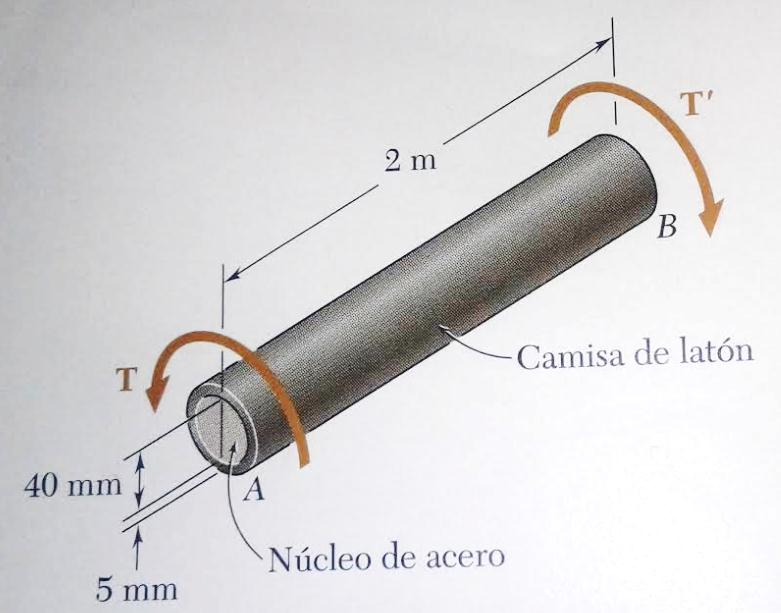
\includegraphics[width=0.4\textwidth]{img/p1.jpg}
\end{center}

\textbf{2.} Para el eje compuesto del problema anterior, el esfuerzo cortante permisible en la camisa de 
latón es de 20 MPa y 45 MPa en el núcleo de acero. Determine a) el par de torsión máximo que puede 
aplicarse al eje, b) el ángulo de giro correspondiente de B respecto a A. \\

\textbf{3.} La figura muestra una barra cilíndrica sólida de acero de 2 in de diámetro empotrada en C y sometida a 
los torques $T_A$ y $T_B$. a) Determine el esfuerzo cortante máximo en los segmentos AB y BC del cilindro 
y (b) calcule el ángulo de giro del extremo A. Utilice $G=12x10^6$ psi.

\begin{center}
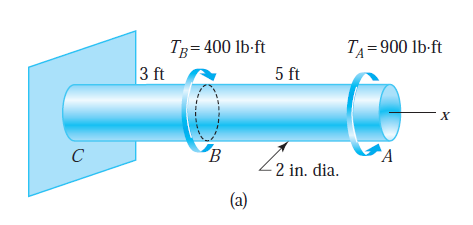
\includegraphics[width=0.55\textwidth]{img/p3.PNG}    
\end{center}

\textbf{4.} Un eje sólido de acero de una roladora transmite 20 kW de potencia a 2 Hz. Calcule 
el diámetro mínimo permisible del eje si el esfuerzo cortante no debe exceder 40 MPa y el 
ángulo de giro está limitado a 6° en una longitud de 3 m. Utilice G=83 GPa. \\ 

\textbf{5.} Un torque T es aplicado a un eje cónico AB como se muestra en la figura. Demuestre 
por integración que el ángulo de giro en A es:

$$ \phi = \frac{7TL}{12\pi G c^4} $$

\begin{center}
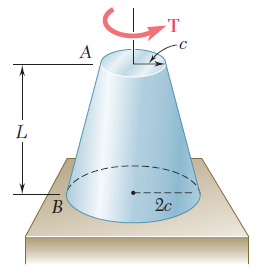
\includegraphics[width=0.28\textwidth]{img/p5.PNG}
\end{center}

\textbf{6.} Dos ejes, cada uno de diámetro de 7/8 in, están conectados por engranes como se muestra 
en la figura. Sabiendo que G = 11.2x10$^6$ psi y que el eje en F está fijo, determine el ángulo de giro 
en A cuando se aplica un par de torsión de 1.2 kip $\cdot$ in en A, tal como se muestra en el esquema.

\begin{center}
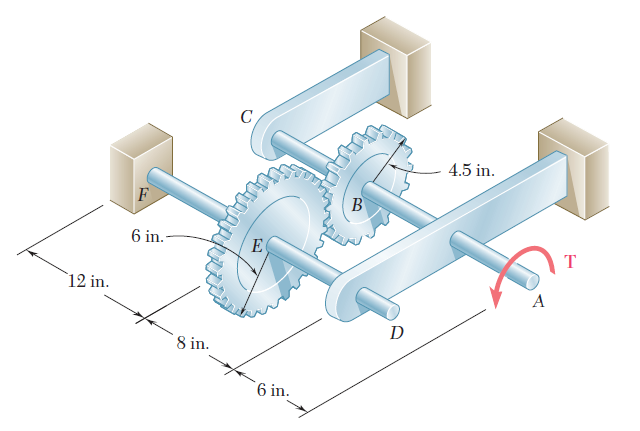
\includegraphics[width=0.65\textwidth]{img/p6.PNG}
\end{center}

\textbf{7.} Al desmontar una rueda para cambiar un neumático,
un conductor aplica fuerzas P = 25 lb en los extremos de dos
de los brazos de una llave de cruz (consulte la figura). La llave
está hecha de acero con módulo de elasticidad en cortante
G = 11.4x10$^6$ psi. Cada brazo de la llave tiene una longitud
de 9.0 in y tiene una sección transversal circular sólida con
diámetro d = 0.5 in.

\begin{enumerate}[label=\alph*)]
\item Determine el esfuerzo cortante máximo en el brazo
que gira la tuerca del birlo (brazo A). 
\item Determine el ángulo de torsión (en grados) de este
mismo brazo.
\end{enumerate}

\begin{center}
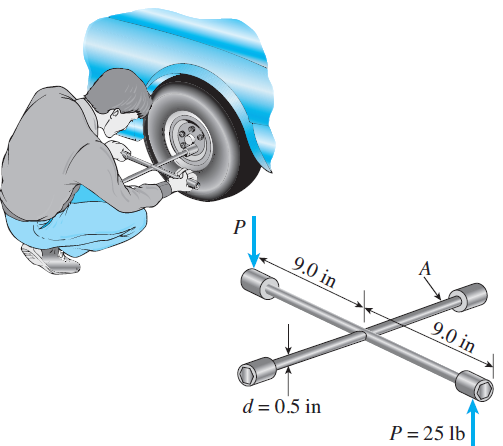
\includegraphics[width=0.5\textwidth]{img/p7.PNG}
\end{center}

\textbf{8.} Cuatro engranes están conectados a un eje circular y
transmiten los pares de torsión que se muestran en la figura. El
esfuerzo cortante permisible en el eje es 10,000 psi.

\begin{enumerate}[label=\alph*,itemsep=1pt]
\item ¿Cuál es el diámetro requerido d del eje si tiene una
sección transversal sólida?
\item ¿Cuál es el diámetro exterior requerido d si el eje es
hueco con un diámetro interior de 1.0 in?
\end{enumerate}

\begin{center}
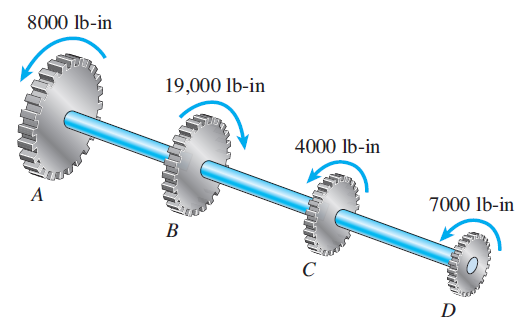
\includegraphics[width=0.55\textwidth]{img/p8.PNG}
\end{center}


\textbf{9.} Un eje escalonado ABCD que consiste en segmentos
circulares sólidos se somete a tres pares de torsión, como se
muestra en la figura. Los pares de torsión tienen magnitudes
de 12.5 kip-in, 9.8 kip-in y 9.2 kip-in. La longitud de cada segmento
es 25 in y los diámetros de los segmentos son 3.5 in, 2.75 in
y 2.5 in. El material es acero con módulo de elasticidad en
cortante G = 11.6x10$^3$ ksi.

\begin{enumerate}[label=\alph*,itemsep=0pt]
\item Calcule el esfuerzo cortante máximo $\tau_{max}$ en el eje.
\item Calcule el ángulo de torsión $\phi_D$ (en grados) en el extremo D.
\end{enumerate}

\begin{center}
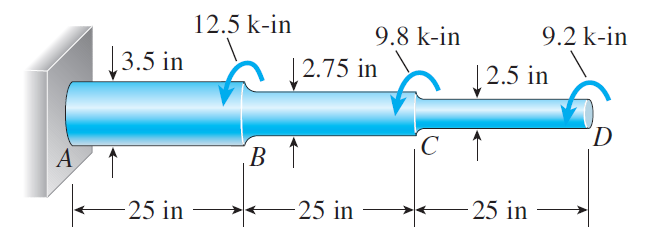
\includegraphics[width=0.55\textwidth]{img/p9.PNG}
\end{center}


\textbf{10.} Un motor suministra 275 hp a 1000 rpm al extremo de
un eje (consulte la figura). Los engranes en B y C toman 125 y
150 hp, respectivamente. Determine el diámetro $d$ requerido del eje si el esfuerzo
cortante permisible es 7500 psi y el ángulo de torsión entre el
motor y el engrane C está limitado a 1.5°. (Suponga G = 11.5x10$^6$ psi, $L_1$ = 6 ft y $L_2$ = 4 ft).

\begin{center}
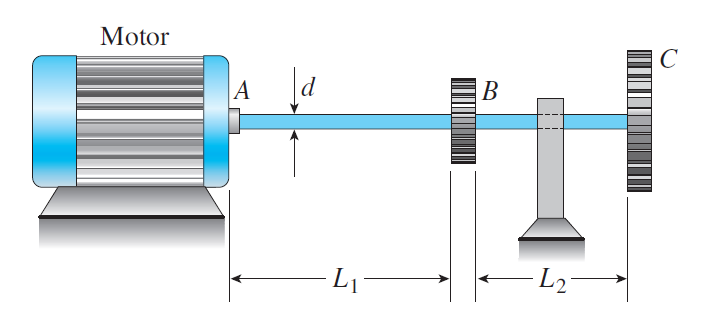
\includegraphics[width=0.55\textwidth]{img/p10.PNG}
\end{center}


\end{document}